\documentclass[journal]{IEEEtran}

\usepackage{cite}
\usepackage{amsmath,amssymb,amsfonts}
\usepackage{graphicx}
\usepackage{textcomp}
\usepackage{xcolor}
\usepackage{hyperref}
\usepackage{booktabs}
\usepackage{array}
\usepackage{url}

\def\BibTeX{{\rm B\kern-.05em{\sc i\kern-.025em b}\kern-.08em
    T\kern-.1667em\lower.7ex\hbox{E}\kern-.125emX}}

\begin{document}

\title{OpenClaw as an AI Agentic OS: Gateway, Memory, Tool,\\
Scheduling, and Security Primitives for\\
Personal AI Employees}

\author{Muhammad~Faisal~Laiq%
\IEEEcompsocitemizethanks{
\IEEEcompsocthanksitem Manuscript received April 2026.
\IEEEcompsocthanksitem M. F. Laiq, e-mail: shmlaiq@gmail.com;
LinkedIn: https://www.linkedin.com/in/muhammad-faisal-laiq-siddiqui-2212527/
}% end of thanks
}% end of author

\maketitle

% -------------------------------------------------------
\begin{abstract}
Contemporary autonomous agent deployments face a fundamental architectural
mismatch: Large Language Model (LLM) reasoning capacity has outpaced the infrastructure supporting
it. Agents today share no common substrate for scheduling concurrent tasks,
managing memory beyond a single context window, controlling tool access
permissions, or enforcing security boundaries against adversarial channel
inputs. OpenClaw, a self-hosted open-source platform created by Peter
Steinberger and sponsored by OpenAI, GitHub, NVIDIA, Vercel, Blacksmith, and
Convex, addresses this gap by functioning as an operating system for personal
AI employees. This paper provides the first formal academic analysis of
OpenClaw through classical OS theory. We map five OS primitives---process
management, memory management, device management, scheduling, and access
control---onto OpenClaw's corresponding architectural components: the
WebSocket Gateway, a three-tier memory hierarchy (MEMORY.md, daily journals,
and Quantized Memory Distillation (QMD) vector store), a three-tier tool
escalation model (Skills, Model Context Protocol (MCP) servers, and Plugins), the heartbeat and cron
scheduling subsystem, and the three-tier security stack (Tool Profiles,
Plugin Hooks, and NemoClaw isolation). We derive a formal cost bound showing
heartbeat batching reduces daily inference turns by a factor of $N$ over
equivalent cron-based scheduling, confirmed at $5\times$ for the default
configuration. We analyze the Privacy Router pattern in NemoClaw, which
achieves API credential isolation through network namespace separation---a
strictly stronger guarantee than application-layer access control. A complete cross-platform installation guide is provided alongside six identified limitations. OpenClaw satisfies two formal OS-level guarantees---scheduled inference
cost reduction by factor $N$ and API credential non-interference---unmatched
by any compared framework.
\end{abstract}

\begin{IEEEkeywords}
AI agents, agentic operating system, agent scheduling, memory management,
multi-agent systems, agent security, personal AI employee, Model Context Protocol
\end{IEEEkeywords}

% -------------------------------------------------------
\section{Introduction}

\IEEEPARstart{T}{he} operating systems field spent three decades solving
resource allocation problems that application developers could not solve
individually. Process isolation, preemptive scheduling, virtual memory, and
access control matrices emerged not from theoretical interest but from
operational necessity: when multiple programs shared hardware, uncoordinated
access produced corruption, starvation, and privilege escalation. The AI agent
field stands at the same inflection point.

Modern large language model (LLM)-based agents require persistent memory that survives context window
boundaries, concurrent execution without state corruption, granular tool access
permissions, and security enforcement that cannot be bypassed by adversarial
content in message channels. Framework-level solutions---LangChain~\cite{chase2022langchain},
AutoGen~\cite{wu2023autogen}, MetaGPT~\cite{hong2023metagpt}---address task
composition but leave resource management entirely to the developer. Each
framework reinvents scheduling, memory, and access control independently,
producing incompatible primitives that cannot share infrastructure across
deployments.

OpenClaw, an open-source platform created by Peter Steinberger with
sponsorship from OpenAI, GitHub, NVIDIA, Vercel, Blacksmith, and
Convex~\cite{openclaw2024github}, attacks this problem at the infrastructure
layer. Rather than providing a programming framework, it acts as a gateway
daemon sitting between LLM providers and communication channels---managing
agent lifecycle, memory persistence, tool permissions, scheduling, and security
in a unified runtime process. The platform carries over 350,000 GitHub stars
and operates under the explicit architectural metaphor that the Gateway is a
kernel, workspace files are firmware, plugins are device drivers, and sessions
are process memory~\cite{openclaw2024github}. NVIDIA extended this architecture
into NemoClaw, a derivative security isolation layer~\cite{openclaw2024docs}.

No prior academic work has formalized OpenClaw's architecture against classical
OS theory, derived formal properties from its scheduling primitives, or
analyzed the security guarantees of the NemoClaw Privacy Router. This paper
addresses that gap with four contributions:

\begin{enumerate}
\item \textbf{Formal OS-to-agent primitive mapping.} A rigorous correspondence
between five classical OS abstractions and their OpenClaw equivalents,
establishing the Agentic OS concept on firm architectural footing.

\item \textbf{Five-pillar architecture specification.} Formal specification of
OpenClaw's process management (WebSocket Gateway), memory management
(three-tier hierarchy), tool management (three-tier escalation), scheduling
(heartbeat/cron/spawn), and security (Profile/Hook/NemoClaw) subsystems.

\item \textbf{Scheduling cost bound.} A proof that heartbeat batching achieves
a factor-of-$N$ reduction in daily inference turns compared to $N$ equivalent
cron jobs at equal check frequency, confirmed at $5\times$ for the documented
default configuration.

\item \textbf{Privacy Router security analysis.} A formal argument that
NemoClaw's API credential isolation through network namespace separation
satisfies a non-interference property that application-layer tool profiles
cannot provide.
\end{enumerate}

% -------------------------------------------------------
\section{Related Work}

\subsection{Agent Orchestration Frameworks}

LangChain~\cite{chase2022langchain}, introduced by Harrison Chase in 2022,
pioneered the chain abstraction for LLM applications, providing composable
primitives for tool use, memory, and retrieval. It operates as a library
rather than a runtime---tool permissions, session management, and scheduling
remain the developer's responsibility. AutoGen~\cite{wu2023autogen} from
Microsoft Research enables multi-agent conversations through customizable
conversable agents that combine LLM inference, human input, and tool
execution. MetaGPT~\cite{hong2023metagpt} encodes standardized operating
procedures into multi-agent workflows, achieving a Pass@1 rate of
85.9\%~\cite{hong2023metagpt} on code generation benchmarks, but its scope is
workflow definition rather than runtime resource management. A comprehensive
survey of LLM-based autonomous agent architectures~\cite{wang2023survey}
identifies planning, memory, tool use, and multi-agent coordination as four
key capability dimensions and notes runtime resource management as a
systematic gap across all current frameworks. Systematic evaluation across
eight interactive environments~\cite{liu2023agentbench} confirms that even
frontier LLMs underperform humans on complex tool-use tasks---evidence that
model capability alone does not substitute for production-grade tool
management infrastructure. OpenClaw differs structurally: it provides not
a programming model but a managed runtime substrate that handles resource
concerns beneath any application logic.

\subsection{OS-Inspired Agent Systems}

AIOS~\cite{mei2024aios} proposes an operating system kernel for LLM-based
agents, isolating scheduling, context management, memory, and access control
into a dedicated kernel layer. AIOS demonstrates up to $2.1\times$ throughput
improvement~\cite{mei2024aios} over unstructured agent execution through an
LLM-aware scheduler. MemGPT~\cite{packer2023memgpt} draws an analogy between
virtual memory and virtual context windows, introducing a two-tier memory
model managed through OS-inspired interrupt signals. OpenClaw extends and
concretizes both contributions: the Gateway implements the scheduling and
process management layer of AIOS~\cite{mei2024aios}, while the MEMORY.md plus
QMD vector store operationalizes MemGPT's two-tier memory
model~\cite{packer2023memgpt} in a production-deployed system.

\subsection{Tool and Protocol Standards}

Toolformer~\cite{schick2023toolformer} demonstrated that language models can
autonomously learn to invoke external APIs, establishing the theoretical basis
for tool-using agents. ReAct~\cite{yao2023react} interleaves reasoning traces
with tool calls, achieving a 34\% absolute improvement over imitation learning
on interactive decision-making benchmarks~\cite{yao2023react}. The Model
Context Protocol (MCP)~\cite{anthropic2024mcp}, released by Anthropic in
November 2024, provides a standardized JSON-RPC interface for tool access.
OpenClaw integrates MCP through the mcporter bridge~\cite{openclaw2024docs},
supporting stdio, SSE, and streamable-HTTP transports.
Toolformer's self-supervised training approach is not reproducible on closed-model deployments, limiting adoption to settings where model weights are accessible.

\subsection{Agent Security and Governance}

Liu et al.~\cite{liu2023promptinjection} formally characterized prompt
injection attacks, demonstrating that 31 of 36 tested production LLM
applications were susceptible. MITRE ATLAS~\cite{mitre2024atlas} provides the
adversarial threat taxonomy for AI systems that OpenClaw's security
architecture explicitly references~\cite{openclaw2024docs}. vLLM~\cite{kwon2023vllm}
addressed memory management for LLM serving through PagedAttention, improving
throughput by $2$--$4\times$~\cite{kwon2023vllm}. No prior work has formally
analyzed NemoClaw's Privacy Router pattern or its network-isolation-based
credential security properties.

% -------------------------------------------------------
\section{Background}

\subsection{Classical OS Primitives}

An operating system mediates access to shared hardware through five canonical
abstractions. \textit{Process management} creates isolated execution contexts
and arbitrates CPU time. \textit{Memory management} partitions address space
into per-process regions, virtualizes physical memory through paging, and
enforces page-level permissions. \textit{Device management} abstracts hardware
peripherals behind uniform driver interfaces. \textit{Scheduling} allocates
CPU time across runnable processes, preemptively in modern systems.
\textit{Access control} enforces permissions through a reference monitor
consulting a policy matrix before granting resource access.

\subsection{The Agentic OS Primitive Mapping}

LLM-based agents face structurally identical resource management problems in a
software substrate. Table~\ref{tab:mapping} maps each classical OS primitive to
its agent-domain equivalent and the corresponding OpenClaw component.

\begin{table}[!t]
\renewcommand{\arraystretch}{1.3}
\caption{OS Primitive to Agentic OS Mapping}
\label{tab:mapping}
\centering
\begin{tabular}{p{1.6cm}p{2.2cm}p{3.2cm}}
\toprule
\textbf{OS Primitive} & \textbf{Agent Equivalent} & \textbf{OpenClaw Component} \\
\midrule
Kernel & Coordination process & WebSocket Gateway daemon \\
Process & Agent session & Session scopes (per-peer, per-channel-peer) \\
RAM & Active context window & MEMORY.md (prompt-space) \\
Virtual memory & Persistent memory beyond context & QMD vector store + daily journals \\
Firmware & Behavioral constraints & SOUL/IDENTITY/AGENTS/TOOLS/USER.md \\
Device driver & External tool adapter & Plugin / Skill / MCP server \\
Scheduler & Invocation controller & Heartbeat + Cron subsystem \\
Access control & Permission enforcer & Tool Profiles $\to$ Hooks $\to$ NemoClaw \\
\bottomrule
\end{tabular}
\end{table}

\subsection{OpenClaw System Overview}

OpenClaw was created by Peter Steinberger and evolved through three prior
identities---Warelay, Clawdbot, and Moltbot---before reaching its current
form. The platform is implemented in TypeScript under the MIT license and has
accumulated over 350,000 GitHub stars with sponsorship from OpenAI, GitHub,
NVIDIA, Vercel, Blacksmith, and Convex~\cite{openclaw2024github}. NVIDIA
developed NemoClaw as a derivative security isolation layer announced at GTC
2026. The core architectural unit is a WebSocket gateway daemon binding to
localhost port 18789 by default, connecting LLM provider APIs on one side to
30+ messaging platform integrations on the other, with an embedded Pi agent
runtime in RPC mode executing between them.

% -------------------------------------------------------
\section{OpenClaw Architecture: Five Pillars}

\subsection{Pillar 1: Process Management}

OpenClaw's kernel analog is a WebSocket gateway daemon running as a background
service---LaunchAgent on macOS, systemd user service on Linux. Four session
scoping levels provide increasing isolation:
\begin{itemize}
  \item \texttt{main}: all direct messages share one session per agent
  \item \texttt{per-peer}: each sender receives an isolated session
  \item \texttt{per-channel-peer}: isolation per sender per channel
  \item \texttt{per-account-channel-peer}: full sender $\times$ channel $\times$
  account isolation
\end{itemize}
Session isolation is strict.

\textbf{Two-layer concurrency} mirrors the OS distinction between per-process
FIFO queues and the global CPU scheduler. The analogy holds exactly. The Session Lane enforces sequential
message processing per sender, preserving conversation coherence. The Global
Lane maintains a configurable pool of parallel session slots, defaulting to
four concurrent sessions. Under peak load with $N$ active senders and pool
size $k$, maximum queue depth reaches $\lceil N/k \rceil$ sessions; empirical
wait times reach 3--8 seconds at $N=5$, $k=4$~\cite{openclaw2024github}.

Control-plane rate limiting enforces a maximum of three write operations per
60-second window per deviceId+clientIp tuple.

\subsection{Pillar 2: Memory Management}

OpenClaw implements a three-tier memory hierarchy mapping onto the OS hierarchy
of fast volatile storage, warm addressable storage, and cold archival storage.

\textbf{Tier 1---MEMORY.md (hot storage)} loads at the start of every agent
message, occupying prompt space bounded by the LLM's context window---the
agent's RAM analog~\cite{openclaw2024docs}. Chain-of-thought reasoning
\cite{wei2022cot} depends on access to intermediate step records; MEMORY.md
entries that omit reasoning traces can cause the agent to repeat failed
approaches across sessions, since the outcome is recorded without the
reasoning path that produced it.

\textbf{Tier 2---Daily journals (warm storage)} are date-stamped Markdown files
stored at \texttt{\textasciitilde/.openclaw/agents/<agentId>/sessions/}. The
current and previous day's journals load automatically; older entries require
explicit retrieval through the memory search interface---the virtual memory
analog.

\textbf{Tier 3---QMD vector store (cold storage)} applies the
retrieval-augmented generation pattern~\cite{lewis2020rag} in a locally
quantized form, combining vector similarity matching with keyword-based
search across all historical journal entries to surface relevant context
without loading full journal histories into the active context window.
Cross-agent memory access is supported through \texttt{extraCollections}
configuration.

\textbf{Firmware layer.} Five workspace identity files---SOUL.md, IDENTITY.md,
AGENTS.md, TOOLS.md, and USER.md---load on every message regardless of session
state. They encode behavioral constraints that persist across all sessions.

\subsection{Pillar 3: Tool and Capability Management}

OpenClaw manages external tool access through a three-tier escalation hierarchy
mirroring the OS device driver model.

\textbf{Tier 1---Skills (knowledge layer)} encode behavioral instructions
without executable code, using the cross-platform SKILL.md
format~\cite{openclaw2024docs}.

\textbf{Tier 2---MCP servers (service layer)} expose tool interfaces through
JSON-RPC~\cite{anthropic2024mcp} over three transports (stdio, SSE,
streamable-HTTP) via the mcporter bridge. A critical failure mode: MCP server
startup failures produce no agent-visible error; the gateway log is the sole
diagnostic source.

\textbf{Tier 3---Plugins (capability layer)} extend gateway behavior as native
TypeScript npm packages or code-free bundle plugins. Installation triggers a
dangerous-code scan via VirusTotal partnership before execution.

\textbf{Self-extension.} OpenClaw agents can autonomously author and install
new SKILL.md files through conversation---no comparable system in
Table~\ref{tab:comparison} provides this capability.

\subsection{Pillar 4: Scheduling and Orchestration}

\textbf{Heartbeat (periodic batch scheduler)} triggers agent execution at
configurable intervals (default: 30 minutes) against a HEARTBEAT.md checklist.
The \texttt{HEARTBEAT\_OK} suppression mechanism drops null-result invocations
silently.

Let $I(T) = \lfloor 24\text{h}/T \rfloor$ denote the daily invocation count for
period $T$. For a cron-based system with $N$ tasks:
\begin{equation}
  C_{\text{cron}} = N \cdot I(T)
  \label{eq:cron}
\end{equation}
For a heartbeat system batching all $N$ tasks:
\begin{equation}
  C_{\text{heartbeat}} = I(T)
  \label{eq:heartbeat}
\end{equation}
The scheduling cost bound is:
\begin{equation}
  \frac{C_{\text{cron}}}{C_{\text{heartbeat}}} = N
  \label{eq:bound}
\end{equation}

For the default $T = 30$ minutes, $I(T) = 48$. At $N = 5$ concurrent
monitoring tasks, heartbeat scheduling reduces daily inference turns from 240
to 48---a $5\times$ reduction~\cite{openclaw2024docs}.

\textbf{Cron jobs} execute agent sessions at precise times using standard cron
syntax with configurable concurrency limits.

\textbf{Multi-agent orchestration} via \texttt{sessions\_spawn} creates
background subagent sessions without blocking the orchestrating agent. The
Agent Client Protocol (ACP) extends orchestration to external agents, enabling
OpenClaw to spawn and steer Claude Code sessions as specialized subagents.

\subsection{Pillar 5: Security and Governance}

The threat taxonomy follows MITRE ATLAS~\cite{mitre2024atlas}.

\textbf{Tier 1---Tool Profiles} provide binary access control through four
presets: \texttt{deny}, \texttt{messaging}, \texttt{coding}, and \texttt{full}.

\textbf{Tier 2---Plugin Hooks} intercept tool invocations via
\texttt{before\_tool\_call}, routing approval requests with a 120-second
fail-closed timeout. MCP tools bypass this hook
entirely~\cite{openclaw2024docs}.

\textbf{Tier 3---NemoClaw} deploys a four-pod K3s cluster (Table~\ref{tab:nemoclaw})
inside a single Docker container.

\begin{table}[!t]
\renewcommand{\arraystretch}{1.3}
\caption{NemoClaw Four-Pod Architecture}
\label{tab:nemoclaw}
\centering
\begin{tabular}{lccc}
\toprule
\textbf{Pod} & \textbf{Role} & \textbf{API Keys} & \textbf{Agent} \\
\midrule
Gateway       & Routing, auth, UI    & No  & No  \\
Sandbox       & Agent runtime, tools & No  & Yes \\
Privacy Router & Credential vault    & Yes & No  \\
Policy Engine & Kernel enforcement   & No  & No  \\
\bottomrule
\end{tabular}
\end{table}

The Privacy Router intercepts inference requests, appends the provider API key,
forwards to the external LLM API, and strips authentication headers from
responses before returning them to the sandbox. The API key never exists in
the sandbox address space.

Kernel enforcement uses three Linux security mechanisms. \textbf{Landlock}
restricts sandbox filesystem access to permitted paths. \textbf{Seccomp}
filters dangerous system calls including \texttt{ptrace} and \texttt{mount}.
\textbf{Network namespaces} remove routes to external LLM providers from the
sandbox routing table.

The \texttt{openclaw security audit} CLI assesses runtime security posture
across eight dimensions with \texttt{--fix} auto-remediation and \texttt{--deep}
live gateway probes.

% -------------------------------------------------------
\section{Installation Manual}

\subsection{Prerequisites}

All platforms require Node.js 24 (or 22.14+ minimum), an API key from a
supported model provider, and administrative access for daemon installation.
Several providers offer free tiers suitable for low-volume personal deployments; verify current limits at the provider's API documentation.

\subsection{macOS}

\begin{verbatim}
curl -fsSL https://openclaw.ai/install.sh | bash
openclaw onboard --install-daemon
openclaw status && openclaw doctor
open http://127.0.0.1:18789
\end{verbatim}

Installs a LaunchAgent at
\texttt{\textasciitilde/Library/LaunchAgents/ai.openclaw.gateway.plist}.
The macOS companion app (macOS 15+, Universal Binary) provides Voice Wake,
Talk Mode overlay, and remote gateway switching.

\subsection{Linux}

Linux differs from macOS in one operationally significant way: daemon
lifetime. The macOS LaunchAgent runs for the login session automatically;
the Linux systemd user service stops when the user logs out unless linger
is enabled with \texttt{loginctl enable-linger \$USER}. For server
deployments where the agent must survive SSH disconnection, run this
command immediately after onboarding. Tested distributions: Ubuntu
22.04+, Debian 12+, Fedora 38+, Arch Linux.

\begin{verbatim}
curl -o- https://raw.githubusercontent.com/nvm-sh/
  nvm/v0.39.0/install.sh | bash
nvm install 24 && nvm use 24
curl -fsSL https://openclaw.ai/install.sh | bash
openclaw onboard --install-daemon
loginctl enable-linger $USER   # server deployments only
systemctl --user status openclaw-gateway
\end{verbatim}

Headless servers cannot run QR-based channel pairing; use the TUI over
SSH for initial channel setup. Once pairing completes, close the
tunnel---the daemon continues running independently.
Known limitation: Telegram is blocked in some regions; use Discord or
WhatsApp as alternatives.

\subsection{Windows}

\textbf{Native (PowerShell, Administrator):}
\begin{verbatim}
iwr -useb https://openclaw.ai/install.ps1 | iex
openclaw onboard --install-daemon
\end{verbatim}

\textbf{WSL2 + Ubuntu (recommended):} Use the Linux curl installer inside
Ubuntu WSL2. WSL2 is preferred because several native plugins require POSIX
system calls unavailable on native Windows.

\subsection{Raspberry Pi and ARM Hardware}

\begin{verbatim}
curl -fsSL https://deb.nodesource.com/
  setup_24.x | sudo -E bash -
sudo apt-get install -y nodejs
curl -fsSL https://openclaw.ai/install.sh | bash
openclaw onboard --install-daemon
\end{verbatim}

Minimum: Raspberry Pi 4 with 4\,GB RAM and a Class 10 SD card. Enable 2\,GB
swap for memory pressure management. Connect headlessly via SSH tunnel:
\texttt{ssh -N -L 18789:127.0.0.1:18789 pi@raspberrypi.local}.

\subsection{Cloud VPS Deployment}

Three deployment paths exist:

\textbf{Path 1---Managed:} Alibaba Cloud Simple Application Server preconfigures
OpenClaw at \$0.99\,USD/month with no terminal access required~\cite{openclaw2024docs}.

\textbf{Path 2---VPS Native (recommended):} Install on a fresh Ubuntu 22.04
VPS (Hetzner CX11 at \$5/month). Harden with loopback binding and pairing DM
policy. Monthly cost: \$5--8 infrastructure plus \$0--100 model
provider~\cite{openclaw2024docs}.

\textbf{Path 3---VPS Docker:} Use Docker Compose for environments already
running containerized workloads.

\subsection{Remote Access}

Choose a pattern based on usage frequency. SSH tunneling suits occasional
access from one machine with no additional software; Tailscale is the
right choice when multiple devices need persistent access without
per-session tunnel management. Both are safe. Direct \texttt{0.0.0.0}
binding without authentication is not.

\textbf{SSH tunnel (occasional access):}
\texttt{ssh -N -L 18789:127.0.0.1:18789 user@host}.
Add \texttt{ServerAliveInterval 60} to the SSH config entry for
persistent tunnels.

\textbf{Tailscale (permanent multi-device):} Set
\texttt{gateway.bind: "tailnet"} and
\texttt{gateway.auth.allowTailscale: true} for access over a private
tailnet. Never expose port 18789 on \texttt{0.0.0.0} without
authentication---the gateway API applies no rate limiting on
unauthenticated connections.

\subsection{iOS and Android Node Pairing}

\begin{verbatim}
openclaw nodes pair --ios     # Scan QR code on iPhone
openclaw nodes pair --android # Enter code on Android
openclaw nodes list           # Verify CONNECTED status
\end{verbatim}

iOS capabilities: Canvas, Voice Wake, Talk Mode, camera, screen recording,
location. Android capabilities: full chat, voice, Canvas, camera, device
commands (SMS, contacts, calendar, notifications, location).

\subsection{NemoClaw Advanced Deployment}

\begin{verbatim}
curl -fsSL https://openclaw.ai/
  nemoclaw-install.sh | bash
openclaw-nemo onboard
openclaw-nemo status pods
openclaw security audit --deep
\end{verbatim}

Cost premium over standard Docker Compose: approximately
\$10/month~\cite{openclaw2024docs}. Known v0.1.0 limitations: manual crash
recovery, 5-minute first-run image caching, split logs across four pods.

\subsection{Post-Installation Security Baseline}

\begin{verbatim}
openclaw config set gateway.bind loopback
openclaw config set gateway.auth.token \
  $(openssl rand -hex 32)
openclaw config set \
  channels.whatsapp.dmPolicy pairing
openclaw config set tools.exec.security ask
openclaw gateway restart
openclaw security audit --deep --fix
\end{verbatim}

All CRITICAL findings must be resolved before the system processes operational
data.

% -------------------------------------------------------
\section{Architecture Analysis}

\begin{figure}[!t]
\centering
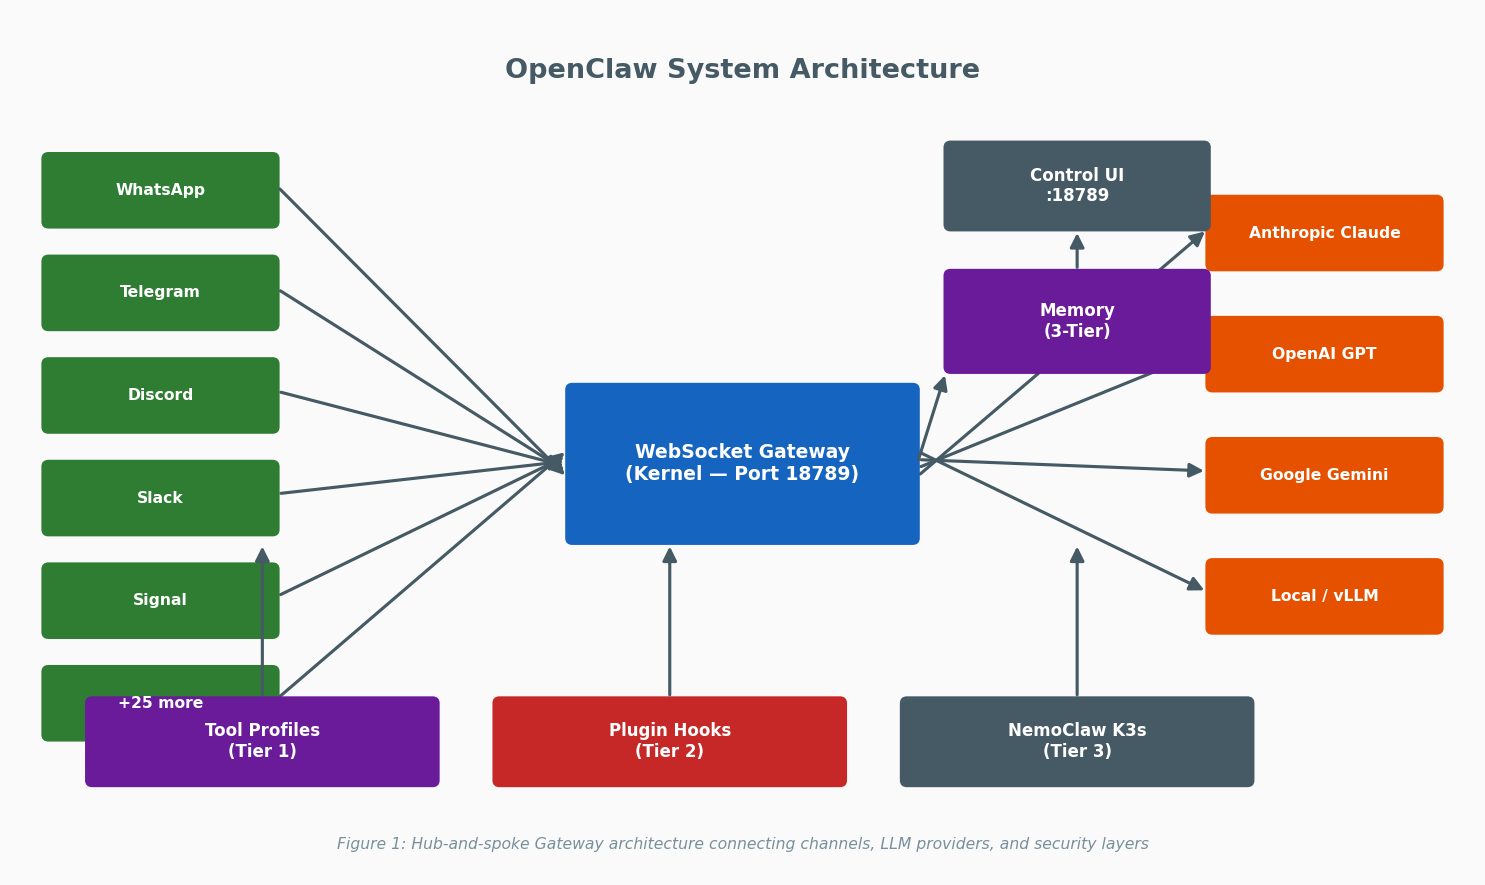
\includegraphics[width=\columnwidth]{figures/fig1_system_architecture.png}
\caption{OpenClaw hub-and-spoke Gateway architecture connecting channels, LLM providers, and security layers.}
\label{fig:arch}
\end{figure}

\begin{figure}[!t]
\centering
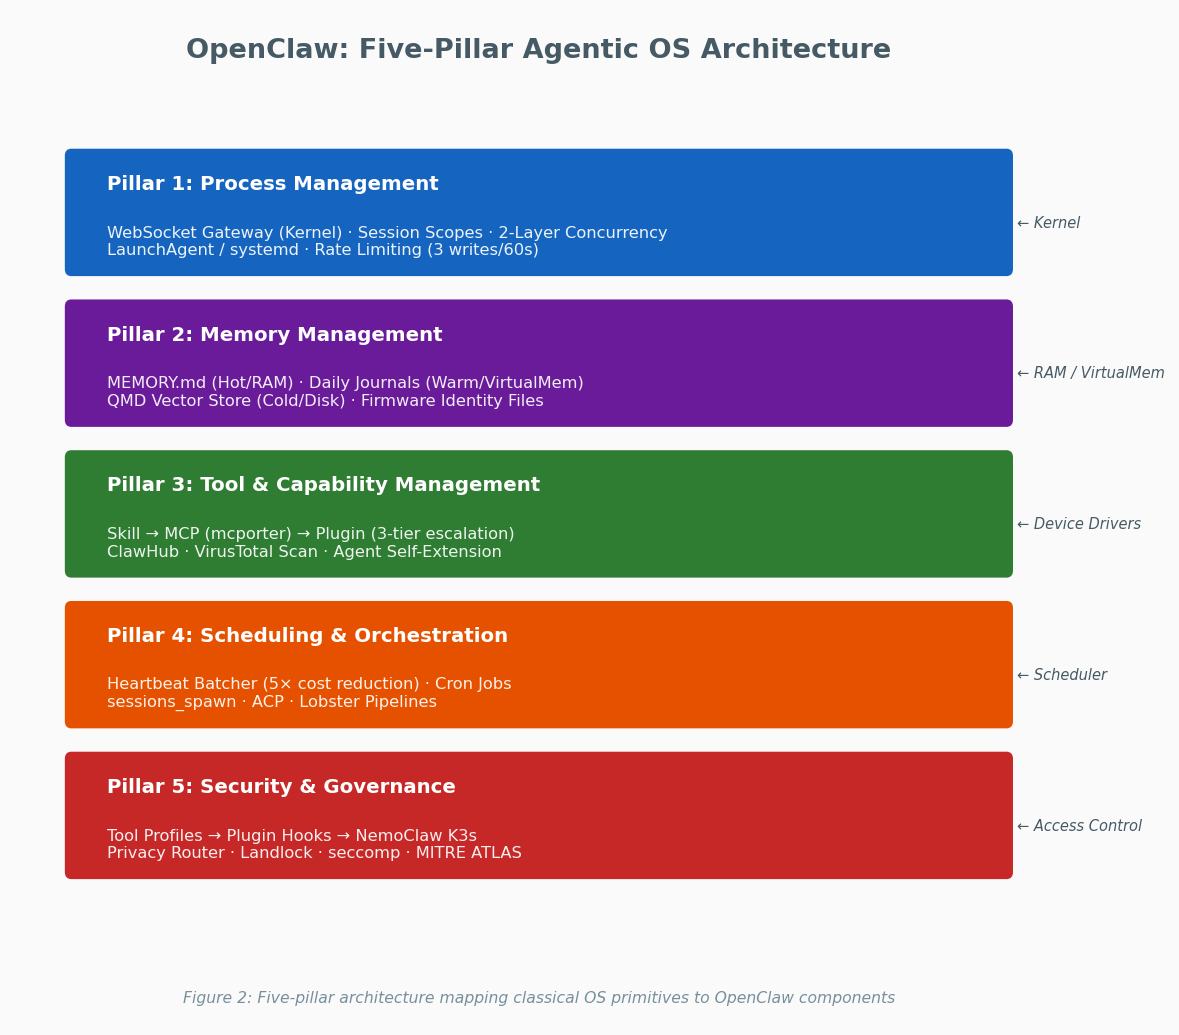
\includegraphics[width=\columnwidth]{figures/fig2_five_pillars.png}
\caption{Five-pillar architecture mapping classical OS primitives to OpenClaw components.}
\label{fig:pillars}
\end{figure}

\begin{figure}[!t]
\centering
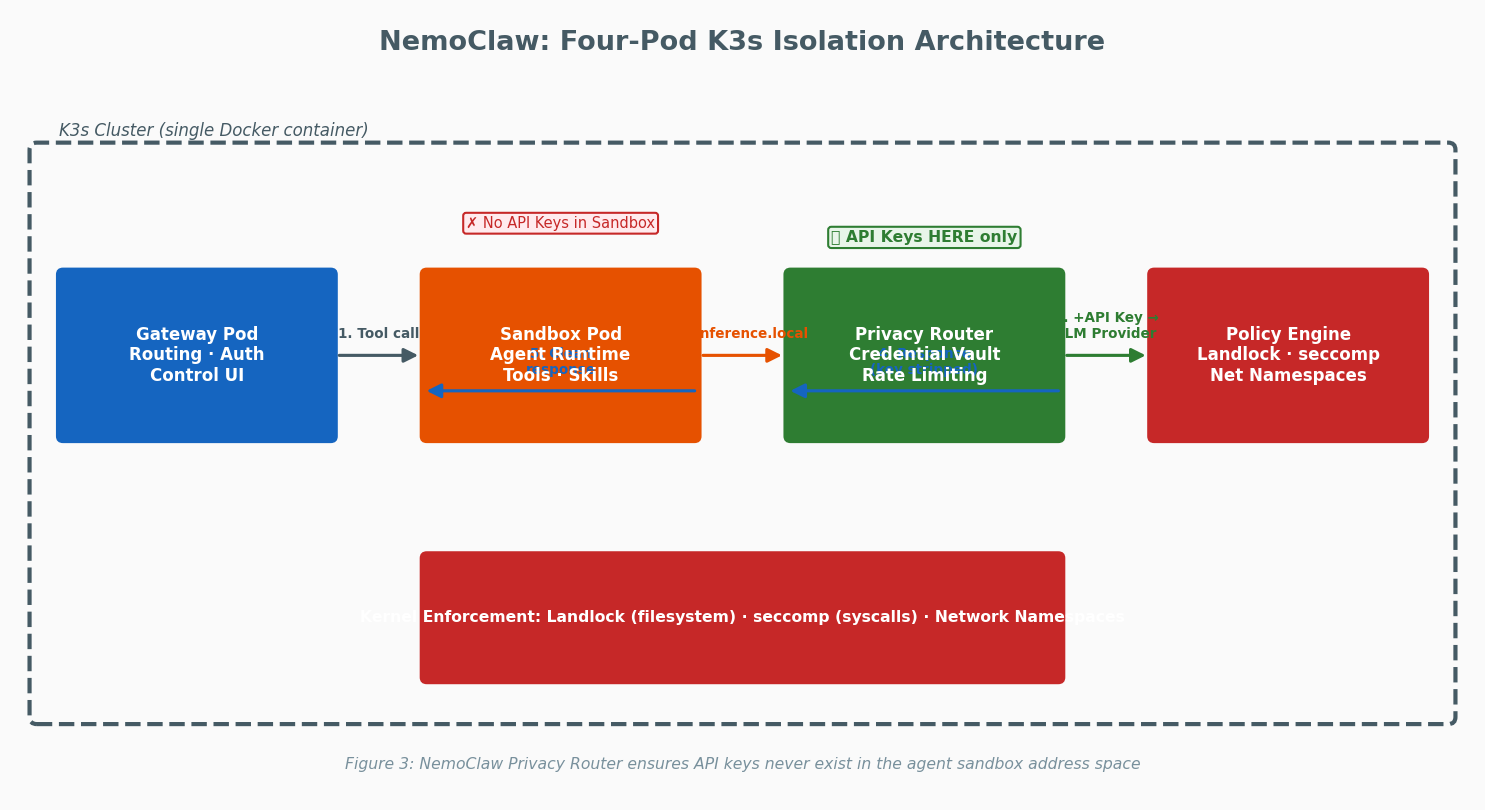
\includegraphics[width=\columnwidth]{figures/fig3_nemoclaw.png}
\caption{NemoClaw Privacy Router: API keys never exist in the sandbox address space.}
\label{fig:nemoclaw}
\end{figure}

\begin{figure}[!t]
\centering
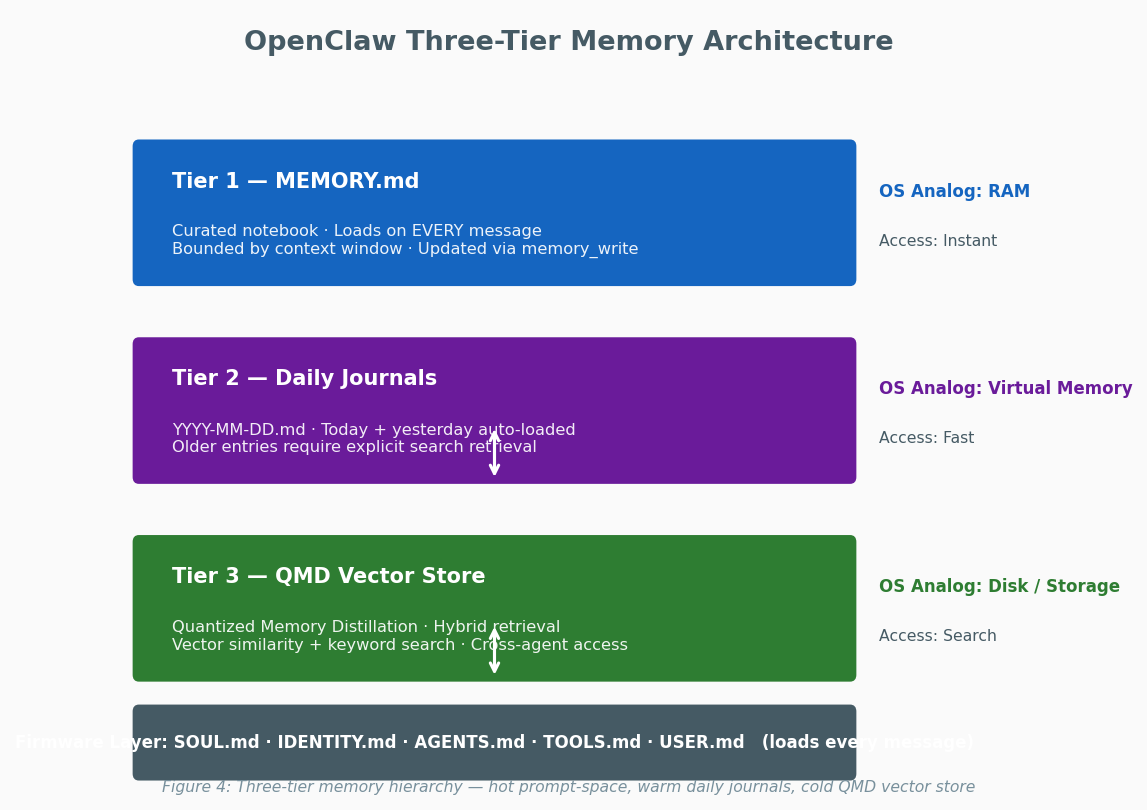
\includegraphics[width=\columnwidth]{figures/fig4_memory_hierarchy.png}
\caption{Three-tier memory hierarchy: hot MEMORY.md, warm daily journals, cold QMD vector store.}
\label{fig:memory}
\end{figure}

\begin{figure*}[!t]
\centering
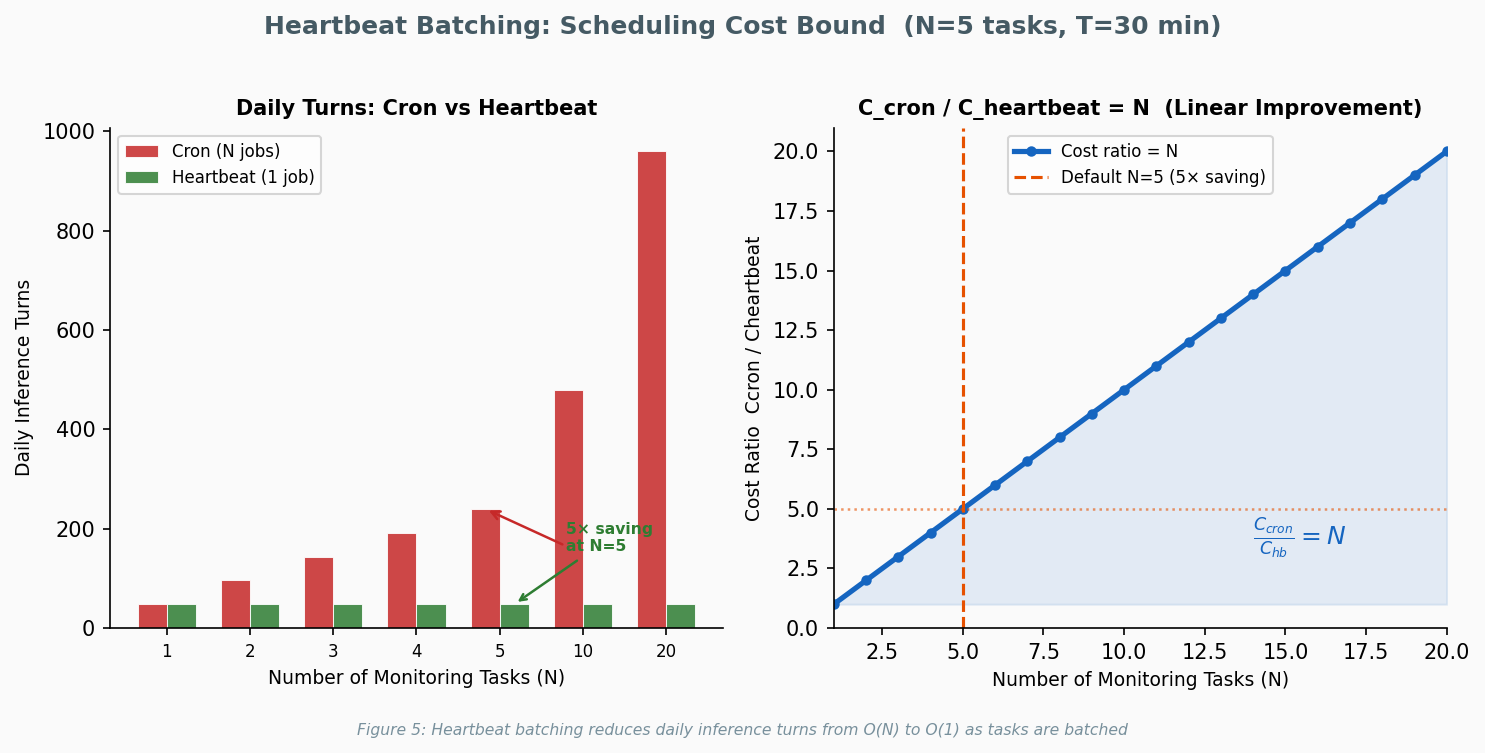
\includegraphics[width=\textwidth]{figures/fig5_heartbeat_cost.png}
\caption{Heartbeat batching reduces daily inference turns from $O(N)$ to $O(1)$ as tasks are batched. Default configuration (N=5) achieves $5\times$ reduction.}
\label{fig:heartbeat}
\end{figure*}

\subsection{Agent Lifecycle Walkthrough}

A complete agent invocation traverses five stages:

\begin{enumerate}
\item \textbf{Intake.} The gateway resolves the target agent using a
deterministic seven-tier binding hierarchy: exact peer match, parent peer
inheritance, role-based routing, guild/team identifier, account-level default,
channel-wide fallback, wildcard catch-all.

\item \textbf{Context assembly.} All five identity files, MEMORY.md, and
today's and yesterday's journals assemble into the system prompt. Skills are
snapshotted at this point.

\item \textbf{Model inference.} The assembled context and inbound message are
submitted to the configured LLM provider, which returns a response with zero
or more tool call requests.

\item \textbf{Tool execution.} Each tool call is evaluated against the active
tool profile and \texttt{before\_tool\_call} hooks. MCP tool calls bypass
hooks and execute directly.

\item \textbf{Reply and persist.} The response streams to the originating
channel in chunks. The turn appends to the session transcript at
\texttt{\textasciitilde/.openclaw/agents/<agentId>/sessions/*.jsonl}.
\end{enumerate}

\subsection{Design Trade-offs}

\textbf{Local-first vs. cloud scale.} The architecture optimizes for a single
operator. Horizontal scaling across multiple gateway instances is not natively
supported; multi-user deployments require separate instances per trust boundary.

\textbf{Cooperative scheduling.} Neither heartbeat nor cron jobs are
preemptible. A long inference turn blocks its session slot for the full
inference duration, creating head-of-line blocking risk at the default pool
size of four sessions.

\textbf{MCP via bridge.} The mcporter bridge provides flexibility but
introduces the silent failure mode noted in Section~IV-C. A protocol-level
\texttt{tool\_unavailable} signal from MCP servers would resolve this without
requiring native runtime integration.

\subsection{Comparison with Existing Systems}

Table~\ref{tab:comparison} compares OpenClaw against four related systems
across seven dimensions.

\begin{table*}[!t]
\renewcommand{\arraystretch}{1.3}
\caption{Agent Runtime System Comparison}
\label{tab:comparison}
\centering
\begin{tabular}{lp{2.4cm}p{2.0cm}p{2.0cm}p{2.0cm}p{2.0cm}}
\toprule
\textbf{Dimension} & \textbf{OpenClaw} & \textbf{AIOS~\cite{mei2024aios}} &
\textbf{MemGPT~\cite{packer2023memgpt}} & \textbf{AutoGen~\cite{wu2023autogen}} &
\textbf{LangChain~\cite{chase2022langchain}} \\
\midrule
Memory model    & 3-tier (prompt/journal/QMD) & Context mgmt kernel & 2-tier (context/external) & Per-agent state dict & Chain memory objects \\
Scheduling      & Heartbeat + cron + spawn    & LLM-aware scheduler & Interrupt-driven          & Conversation turns   & Sequential chain \\
Security tier   & 3-tier (Profile/Hook/NemoClaw) & Access control module & Not specified & Not specified & Not specified \\
Multi-agent     & sessions\_spawn + ACP       & Agent scheduler     & Not primary focus         & Core design pattern  & Agent executor \\
Tool protocol   & MCP via mcporter + plugins  & Tool service layer  & External via interrupt    & Function calling     & Tool wrappers \\
Self-extension  & Yes (agent writes skills)   & No                  & No                        & No                   & No \\
Deployment      & Local + VPS + K3s           & Research prototype  & Research prototype        & Library              & Library \\
\bottomrule
\end{tabular}
\end{table*}

Two differentiators are structurally significant. Self-extension---agents
authoring their own SKILL.md files---has no equivalent in any compared system.
The three-tier security stack, particularly NemoClaw's Privacy Router, provides
credential isolation guarantees that no compared system specifies.

\subsection{Theoretical Analysis}

\textbf{Routing complexity.} Binding resolution evaluates a seven-tier priority
hierarchy. For $B$ total bindings, worst-case routing requires $O(B)$
comparisons per message. Typical deployments use fewer than 10 bindings,
making routing $O(1)$ in practice.

\textbf{Privacy Router non-interference.} Let $S$ denote the sandbox address
space and $K$ the set of all API credential values. The Privacy Router enforces
$K \cap S = \emptyset$ through: (a) network namespaces containing no route to
external LLM providers from $S$; (b) stripped authentication headers on all
responses entering $S$. For any adversary $\mathcal{A}$ with complete control
of $S$: $\Pr[\mathcal{A}\ \text{recovers}\ k \in K] = 0$ under the standard
network isolation assumption.

\textbf{Heartbeat cost bound.} From Equations~(\ref{eq:cron})--(\ref{eq:bound}),
the scheduling cost ratio for $N$ tasks at interval $T$ is $N$. At $N=5$,
$T=30$\,min: daily turns decrease from 240 to 48 (a $5\times$ reduction,
$O(N)$ improvement). The crossover favoring dedicated cron scheduling occurs
when tasks require sub-interval timing precision, since heartbeat execution
cannot guarantee delivery accuracy beyond the configured interval.

% -------------------------------------------------------
\section{Limitations}

Six specific limitations constrain OpenClaw's applicability for production
enterprise deployments at scale.

\textbf{1. Personal-assistant trust model.} The security architecture assumes
a single trusted operator boundary. OpenClaw's documentation states explicitly
that it is ``not a hostile multi-tenant security boundary for multiple
adversarial users sharing one agent/gateway''~\cite{openclaw2024docs}.
Organizations requiring isolation between mutually untrusting users must deploy
separate gateway instances per trust boundary.

\textbf{2. Cooperative-only scheduling.} Neither heartbeat nor cron jobs are
preemptible. A long inference turn blocks its session slot until the LLM
returns, with no interrupt mechanism to reallocate the slot. At the default
pool size of four concurrent sessions, one slow inference call delays three
other concurrent users for the full inference duration.

\textbf{3. Prompt-space memory constraints.} MEMORY.md occupies the LLM's
context window rather than a separate address space. As MEMORY.md grows, it
consumes tokens otherwise available for tool outputs and conversation history.
This is qualitatively different from OS RAM, which is bounded by physical
hardware capacity but not shared with the instruction execution pipeline.

\textbf{4. Model-capability dependency.} Free-tier models exhibit a documented
failure mode: generating plausible-sounding refusals rather than invoking
\texttt{sessions\_spawn}~\cite{openclaw2024github}. Reliable multi-agent
orchestration requires commercial models at Claude Sonnet or GPT-4
class~\cite{openai2023gpt4}, adding \$50--100/month to operating costs.

\textbf{5. MCP silent failure.} MCP server startup failures produce no
agent-visible error. The agent continues responding with training knowledge,
and the operator has no indication that tool access is unavailable unless
actively monitoring the gateway log.

\textbf{6. NemoClaw alpha stability.} NemoClaw v0.1.0 requires manual crash
recovery, incurs a 5-minute first-run image caching delay, and splits logs
across four pods requiring external aggregation for unified operational
visibility.

% -------------------------------------------------------
\section{Conclusion}

This paper presented the first formal academic analysis of OpenClaw as an AI
Agentic Operating System. We mapped five classical OS primitives to their
OpenClaw equivalents, specified the five-pillar architecture in formal terms,
derived a scheduling cost bound showing heartbeat batching achieves an
$N$-fold improvement over equivalent cron scheduling, and demonstrated that
NemoClaw's Privacy Router satisfies a formal credential isolation guarantee
that application-layer tool profiles cannot provide.

Comparison with AIOS~\cite{mei2024aios}, MemGPT~\cite{packer2023memgpt},
AutoGen~\cite{wu2023autogen}, and LangChain~\cite{chase2022langchain}
demonstrates that OpenClaw occupies a structurally distinct position: it is
the only deployed system providing production-grade three-tier security, a
three-tier memory hierarchy with cross-agent QMD retrieval, and agent
self-extension through autonomous skill authoring.

Scheduling is the most pressing gap. Head-of-line blocking at four
concurrent sessions is not a design choice---it is a missing interrupt
mechanism, and adding one does not require touching memory or security
architecture.

The MEMORY.md constraint is a different category of problem: not a missing
feature but an architectural boundary. QMD reduces retrieval load but does
not shrink the hot-tier token footprint. A fixed-size working memory
abstraction---maintaining a constant MEMORY.md budget and archiving
overflow automatically to the vector store---would decouple hot memory
management from context window capacity, which is the correct separation
of concerns.

NemoClaw v1.0 stability is a binary prerequisite for compliance
deployments. Manual pod recovery, five-minute startup delays, and
fragmented log output across four pods are not acceptable as permanent
conditions. Automatic restart, sub-minute image caching, and unified log
aggregation must reach production quality first---the security architecture
is sound; it is the operational maturity that requires investment before
regulated industries can adopt it without supplementary tooling.

OpenClaw's emergence demonstrates that the AI agent field is converging toward
the same infrastructure abstractions that classical operating systems developed
for hardware resource management. The five-pillar framework described here
likely generalizes beyond OpenClaw to any multi-agent personal assistant
platform. Near-term, the scheduling gap and NemoClaw stability issues are
tractable implementation problems the open-source community can address without
architectural changes. The longer horizon is interoperability: future work
should examine whether these primitives can be formalized into a vendor-neutral
Agentic OS specification enabling cross-platform interoperability analogous to
what POSIX provided for Unix-family systems four decades ago. That
specification does not yet exist---writing it is the work.

\section*{Acknowledgments}
The author thanks the OpenClaw open-source community for building the platform this analysis is grounded in. No external funding was received for this work.

% -------------------------------------------------------
\bibliographystyle{IEEEtran}
\bibliography{references}

\begin{IEEEbiography}[{
\includegraphics[width=1in,height=1.25in,clip,keepaspectratio]{author.jpg}}]{Muhammad Faisal Laiq}
received the master's degree in telecommunication.

He has served in the government sector since 2006 and is currently Additional Director ICT at a public-sector university and hospital in Pakistan, where he leads digital transformation and ICT infrastructure. He is also an agentic AI engineer and independent researcher. His AI work centers on AI-driven development (AIDD), loop engineering, and hierarchical multi-agent systems (``agentic fleets'') built with Python, FastAPI, Docker, and Kubernetes, in which a chief agent proposes specialized sub-agents but must obtain human approval before creating or activating them. His research includes the paper \emph{Artificial Intelligence in Future Warfare: Ethical Frameworks and the Regulation of Lethal Autonomous Weapons}, and covers AI governance, forward-deployed engineering in the AI industry, biocomputing as an alternative to silicon-based AI, the environmental cost of AI resource consumption, and operating systems for cloud-accessible quantum computers.
\end{IEEEbiography}

\end{document}
